\documentclass[a4paper]{article}

\usepackage[toc,page]{appendix}

\usepackage[spanish]{babel}
\usepackage[utf8]{inputenc}
\usepackage{amsmath}
\usepackage{graphicx}
\usepackage{fancyhdr}
\usepackage{amsmath}
\usepackage[colorinlistoftodos]{todonotes}
\usepackage{xcolor}
\usepackage{minted}
\usepackage[font=small,labelfont=bf]{caption}
\usepackage{enumitem}
\usepackage{textcomp}
\usepackage{siunitx}
\usepackage{textgreek}
\usepackage{bigints}
\usepackage{amsfonts}

\usepackage{hyperref}

\hypersetup{
    colorlinks,
    citecolor=blue,
    filecolor=blue,
    linkcolor=blue,
    urlcolor=blue
}

\usepackage{geometry}
\geometry{a4paper}

\begin{document}
\begin{figure}
\centering
\includegraphics[scale=1]{./img/logo-facu}
\end{figure}

\title{\large\textsc{66.61 - Tecnología de Circuitos Integrados}\\
\large Trabajo Práctico Final\\
Sintetizador de Frecuencias para un Microcontrolador con un PLL Digital}

\author{
Andrew Parlane \\
}

\maketitle

\newpage

\tableofcontents

\listoffigures

\newpage

\section{Objetivo}

El objetivo de este trabajo es diseñar un sintetizador de frecuencias para uso en un microcontrolador con un PLL digital. Debería tomar un reloj de entrada con frecuencia $f_{ref}$ y unas señales de control y producir un reloj de salida con frecuencia $f_{o} = N f_{ref} / M$, donde N y M depende en las señales de control.

\section{TSMC 180}

Para comenzar tuve que aprender un poco sobre la tecnologia de TSMC 180. Leyendo los documentos dados encontré:

\begin{tabular}{l r}
    Parámetro & Valor \\ \hline
    $L_{MIN}$ & \SI{0.18}{\micro\meter} \\
    $W_{MIN}$ & \SI{0.42}{\micro\meter} \\
    $LD_{MIN}$ & \SI{0.48}{\micro\meter} \\
    $V_{DD_{MAX}}$ & \SI{1.8}{\volt} \\
\end{tabular}

No pude encontrar una lista de capacitancias entre cada capa, pero en el spice.lib encontré $t_{OX} = \SI{4.1}{\nano\meter}$, con esto pude calcular $C\prime_{OX} = \SI[per-mode=symbol]{8418}{\atto\farad\per\micro\meter\squared}$.

Realicé una simulación para encontrar el mejor ratio entre $W_N$ y $W_P$. Figura \ref{fig:wpfact_sch} muestra el esquemático y \ref{fig:wpfact_sim} muestra el resultado. Se produce el mejor tiempo de propagación cuando $W_P = 1.5 W_N$. Así en este proyecto uso WPFACT = 1.5.

\begin{figure}[!htb]
\centering
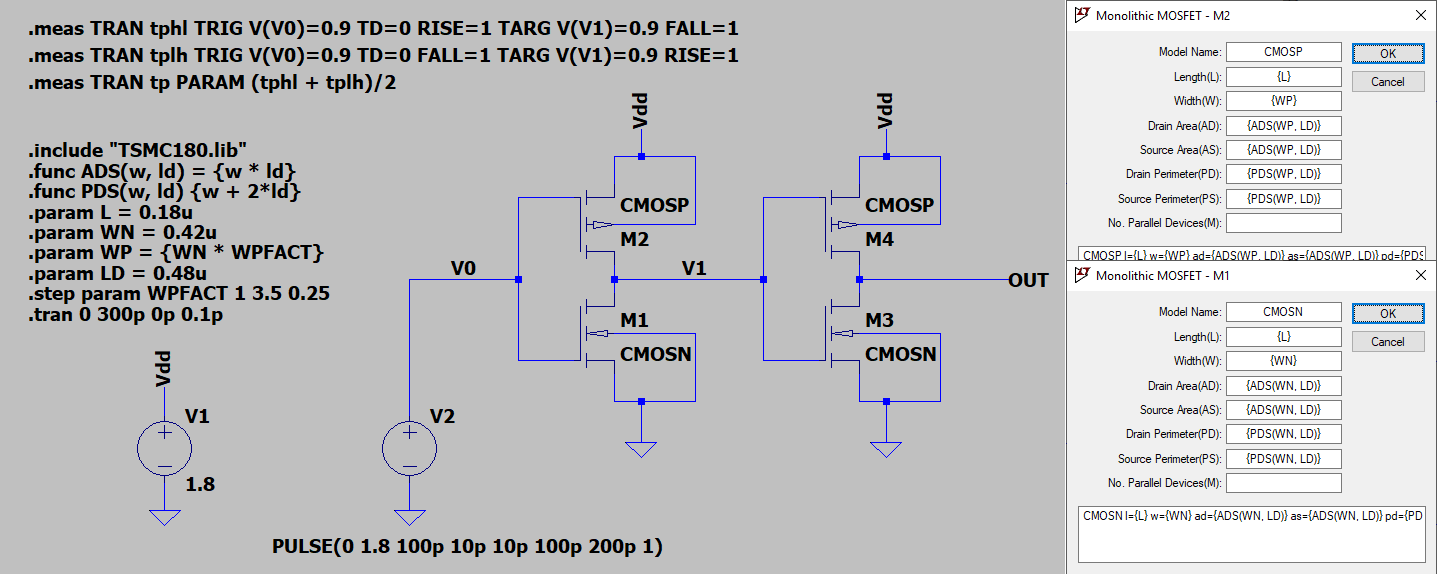
\includegraphics[scale=0.3]{./img/wpfact_sch}
\caption{Esquemático de dos inversores cascadas.}
\label{fig:wpfact_sch}
\end{figure}

\begin{figure}[!htb]
\centering
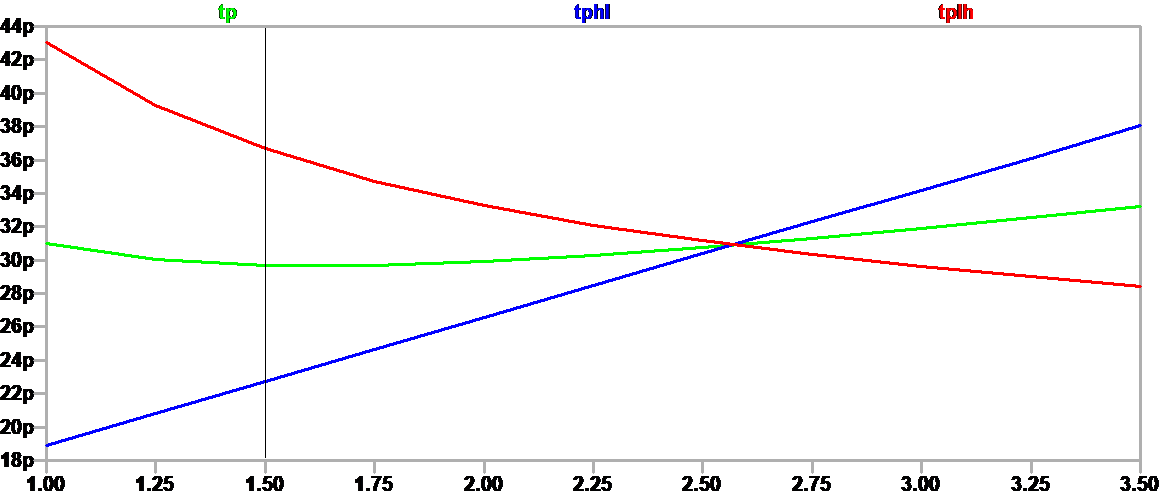
\includegraphics[scale=0.4]{./img/wpfact_sim}
\caption{Simulación para encontrar el mejor ratio entre $W_N$ Y $W_P$}
\label{fig:wpfact_sim}
\end{figure}

\section{Compuertas básicos}

Implementé varias compuertas básicos y realicé simulaciones para verificar su comportamiento. Los componentes que diseñe son:

\begin{itemize}[noitemsep]
    \item AND con 2 entradas.
    \item AND con 3 entradas.
    \item AND con 4 entradas.
    \item FFD con reset asincróno.
    \item Inversor con el drain conectado a $V_{DD}$ y el source conectado a tierra.
    \item Inversor con el drain y el source exportado en el netlist.
    \item MUX con 2 vias.
    \item MUX con 4 vias y salida invertido.
    \item NAND con 2 entradas.
    \item NAND con 3 entradas.
    \item NAND con 4 entradas.
    \item NOR con 2 entradas.
    \item OR con 2 entradas.
    \item Transmission Gate.
    \item XNOR con 2 entradas.
    \item XOR con 2 entradas.
\end{itemize}

No uso todos en mi diseño final. Cada compuerta consiste de un .asc y un .asy, y es parametrizado así que cada instancia puede usar tamaños diferentes. Figura \ref{fig:compuertas_sch} muestra una selección de los compuertas.

\begin{figure}[!htb]
\centering
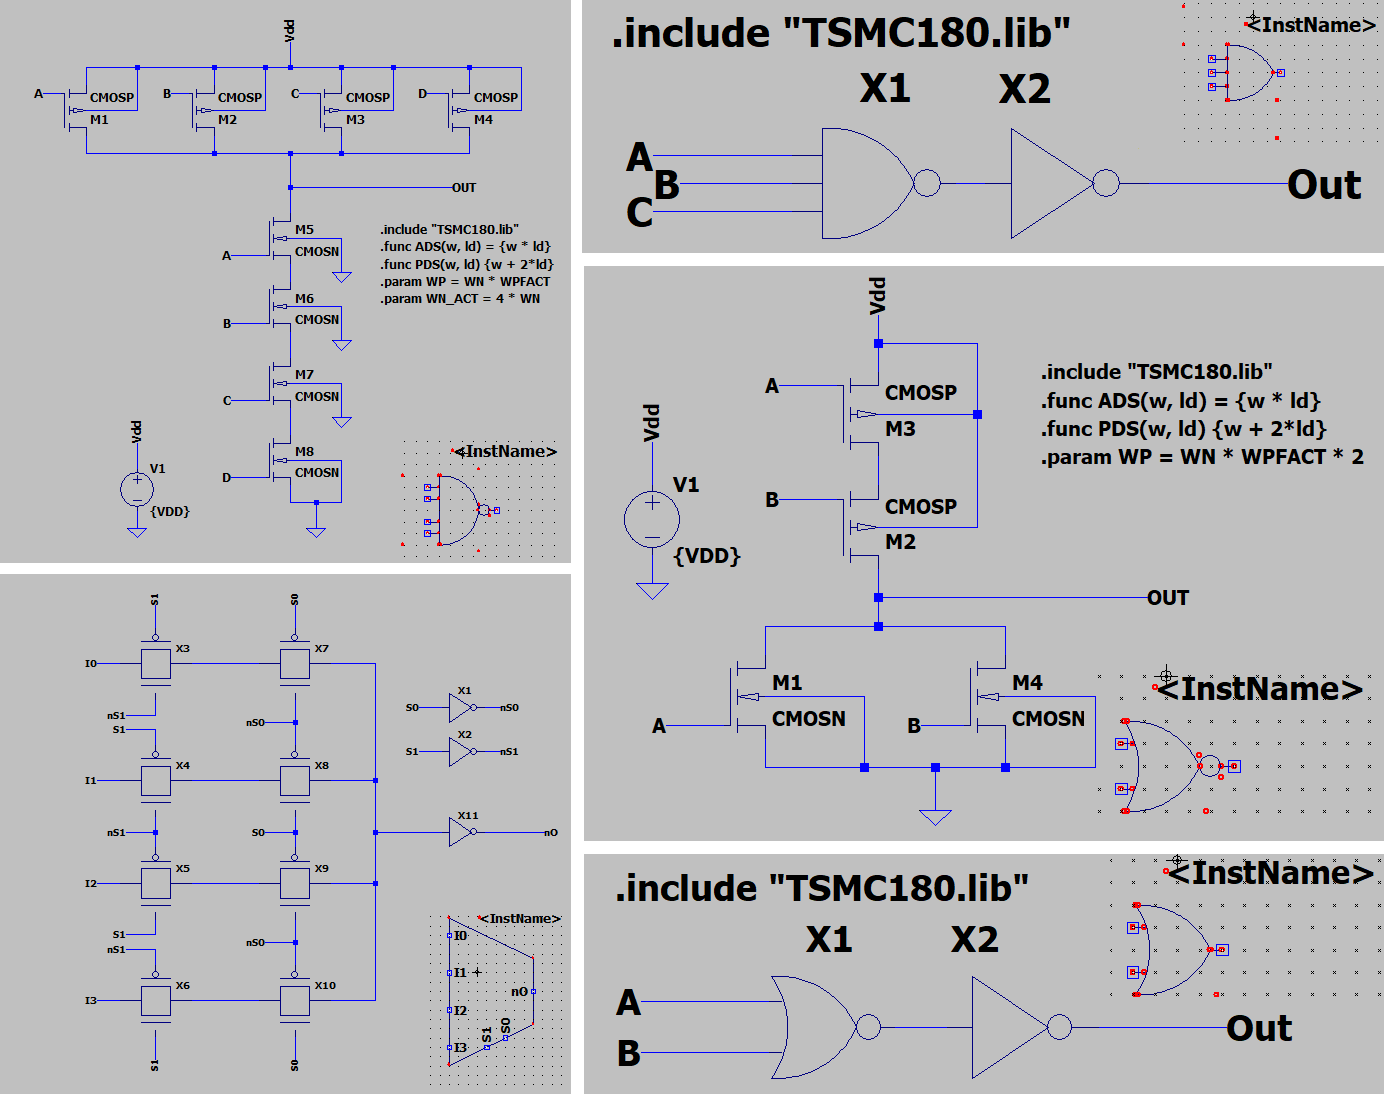
\includegraphics[scale=0.4]{./img/compuertas_sch}
\caption{Una selección de compuertas.}
\label{fig:compuertas_sch}
\end{figure}

\section{VCO}

Hay varias formas construir un VCO (por Voltage Controlled Oscillator), elegí usar un oscilador en anillo limitado por corriente. Figura \ref{fig:csro1} muestra la idea. Funciona cómo un oscilador en anillo normal pero los fuentes de corrientes controlan el tiempo de propagación del inversor, que cambia la frecuencia de operación:

\begin{align*}
C_{tot} &= \frac{5}{2} C\prime_{OX}(W_N L_N + W_P L_P) \\
f &= \frac{I_D}{N C_{tot} V_{DD}}
\end{align*}

Donde N es el número de inversores, en el anillo, y $W_N, L_N, W_P, L_P$ son los anchos y largos de los transistores en los inversores. Elegí una corriente central de \SI{10}{\micro\ampere} que me da por inversores mínimos, y $N = 7$:

\begin{align*}
C_{tot} &= \SI{4.0}{\femto\farad} \\
f &= \SI{198.4}{\mega\hertz}
\end{align*}

\begin{figure}[!htb]
\centering
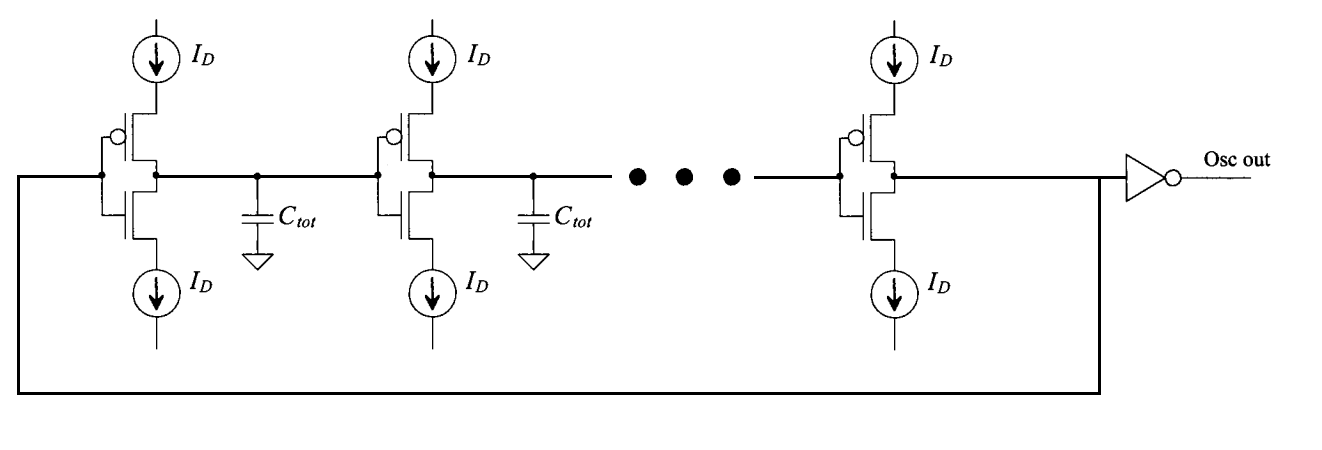
\includegraphics[scale=0.4]{./img/csro1}
\caption{Un Oscilador en Anillo limitado por corriente.}
\label{fig:csro1}
\end{figure}

El primer parte estuvo diseñar una fuente de corriente controlado por una tensión. Figura \ref{fig:current_source_sch} muestra el diseño que usé.

\begin{figure}[!htb]
\centering
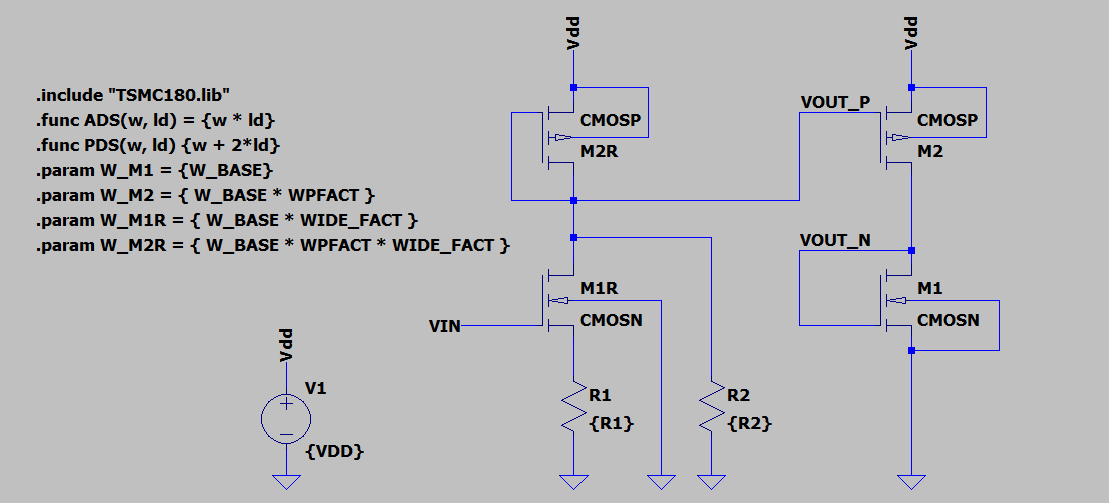
\includegraphics[scale=0.4]{./img/current_source_sch}
\caption{Fuente de corriente controlado por tensión.}
\label{fig:current_source_sch}
\end{figure}

El resistor R1 controla el pendiente de corriente contra tensión de $V_{IN}$. El resistor R2 controla el corriente mínimo cuándo $V_{IN} < V_T$, y los ratios de anchos de los cuatros transistores linearizan la salida.

Después de jugando con las simulaciones encontré los siguiente valores:

\begin{align*}
L &= \SI{0.9}{\micro\meter} \\
W_N &= \SI{4.0}{\micro\meter} \\
WPFACT &= 1.5 \\
WIDE_FACT &= 3 \\
R1 &= \SI{20.0}{\kilo\ohm} \\
R2 &= \SI{86.0}{\kilo\ohm}
\end{align*}

Que me da la salida mostrado en figura \ref{fig:current_source_sim}. Un corriente mínimo de \SI{5.0}{\micro\ampere}, un corriente central de \SI{9.9}{\micro\ampere}, y un corriente máximo de \SI{20.4}{\micro\ampere}. El pendiente es bastante lineal por $V_{IN} > \SI{0.7}{\volt}$, cómo mostrado con la línea azul, con una ecuación de $ I_D = \SI[per-mode=symbol]{11.5}{\micro\ampere\per\volt} V_{IN} - \SI{0.5}{\micro\ampere} $.

\begin{figure}[!htb]
\centering
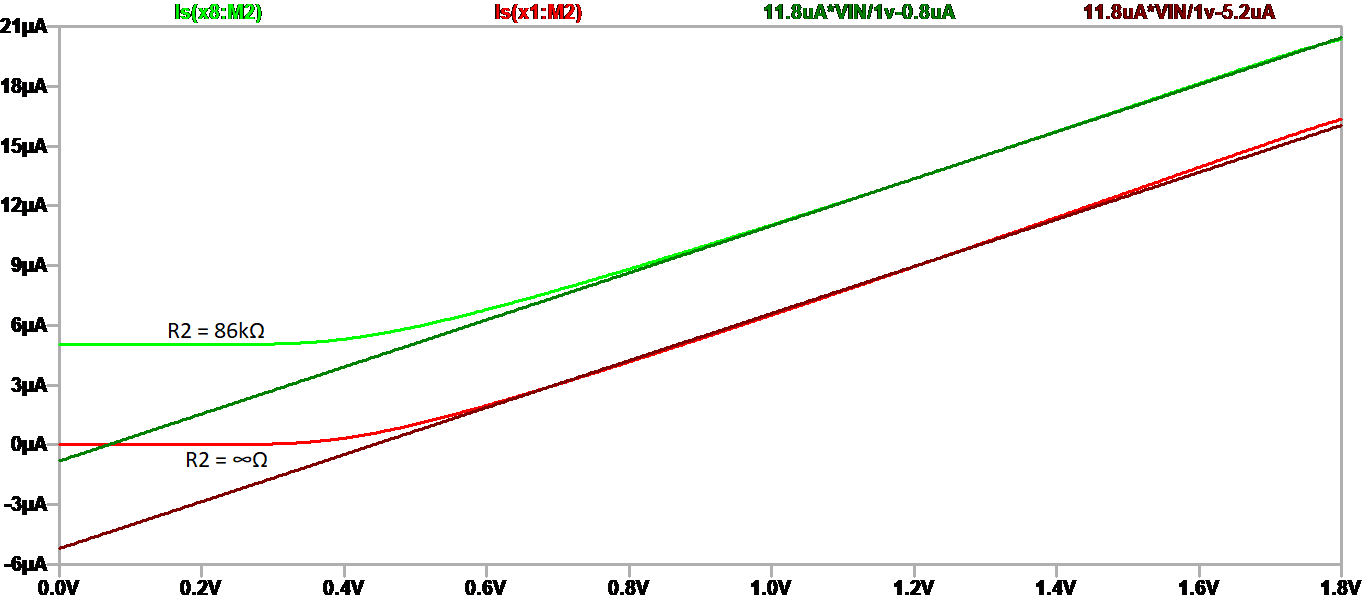
\includegraphics[scale=0.4]{./img/current_source_sim}
\caption{Simulación de la fuente de corriente controlado por tensión.}
\label{fig:current_source_sim}
\end{figure}

Figura \ref{fig:vco7_sch} muestra el esquemático del VCO, y Figura \ref{fig:vco7_test_sch} muestra el esquemático de prueba con todos los parámetros. Uso directivos de SPICE para medir calcular la frecuencia promedio y el duty cycle sobre 100 ciclos. También calculo la frecuencia de salida esperado usando las ecuaciones anteriores. Encontré que la realidad y la teoría están bastante diferentes para inversores mínimos, así realicé una simulación para ver cómo cambiando $W_N$ afecta estos valores con $W_N$. Figura \ref{fig:vco7_sim_wn} muestra el resultado. La frecuencía calculada y medida están iguales por $W_N = \SI{0.57}{\micro\meter} y V_{IN} = \SI{0.9}{\volt}$. Intenté usar este valor pero la simulación estuvo dando me resultos raros por $V_{IN} < \SI{0.5}{\volt}$, así estoy usando $W_N = \SI{0.57}{\micro\meter}$.

\begin{figure}[!htb]
\centering
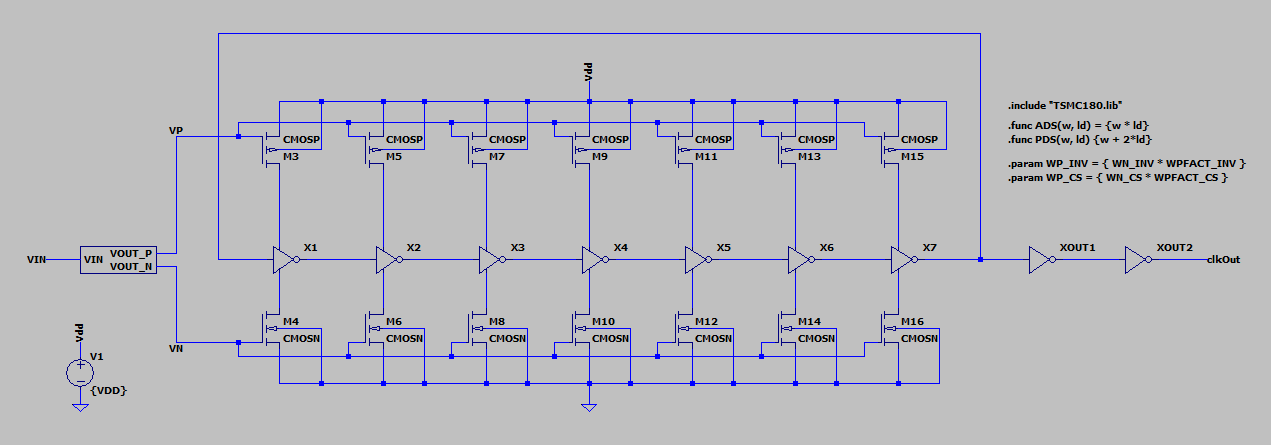
\includegraphics[scale=0.4]{./img/vco7_sch}
\caption{Esquemático del VCO.}
\label{fig:vco7_sch}
\end{figure}

\begin{figure}[!htb]
\centering
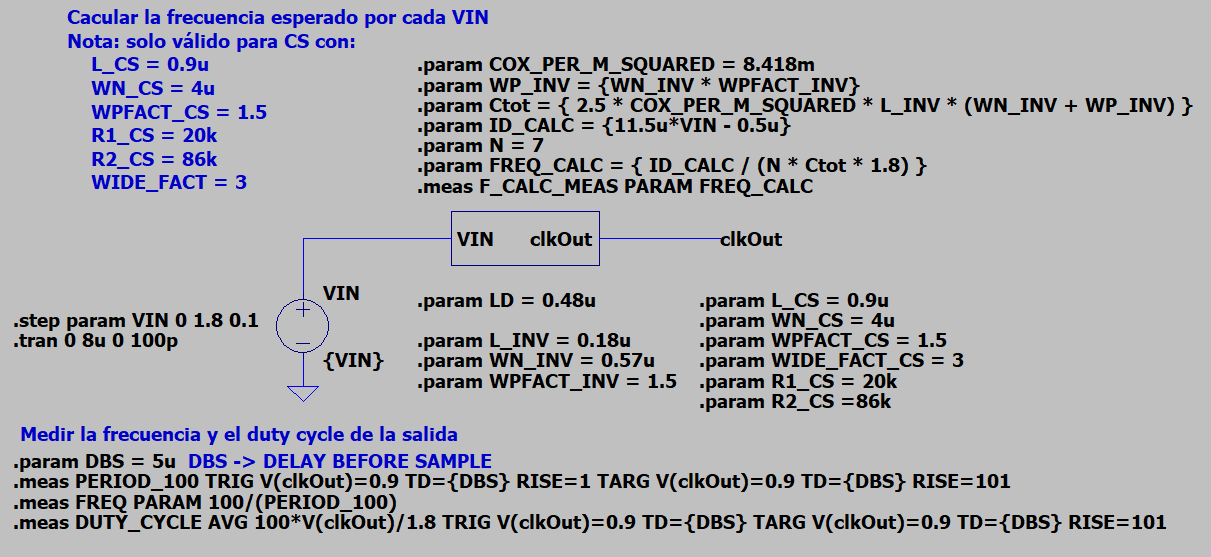
\includegraphics[scale=0.4]{./img/vco7_test_sch}
\caption{Esquemático de la prueba para VCO.}
\label{fig:vco7_test_sch}
\end{figure}

\begin{figure}[!htb]
\centering
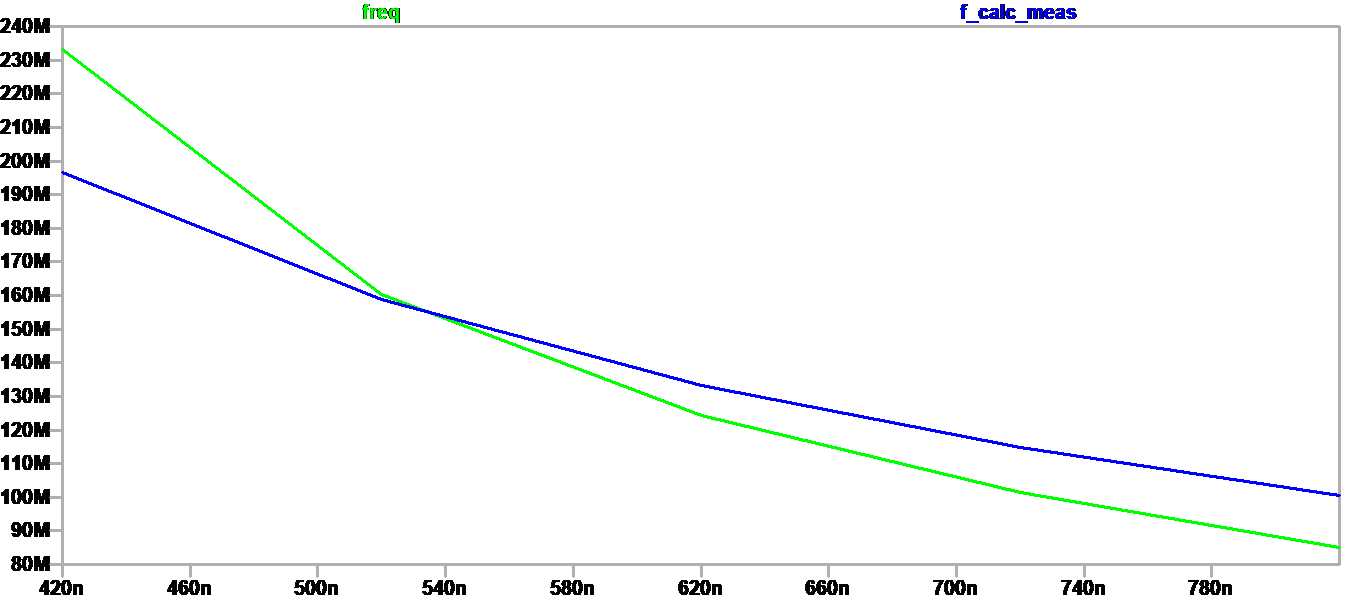
\includegraphics[scale=0.4]{./img/vco7_sim_wn}
\caption{Simulación de Frecuencia medida y estimada contra $W_N$.}
\label{fig:vco7_sim_wn}
\end{figure}

Figura \ref{fig:vco7_sim} muestra cómo cambia la frecuencia medido y estimado con $V_{IN}$. No están iguales pero están bastante cerca. El pendiente del parte lineal es aproximadamente \SI[per-mode=symbol]{200}{\mega\hertz\per\volt} dando un $K_{VCO} = 2\pi \SI[per-mode=symbol]{200}{\mega\hertz\per\volt} = 1,26 * 10^9 radians/Vs$.

\begin{figure}[!htb]
\centering
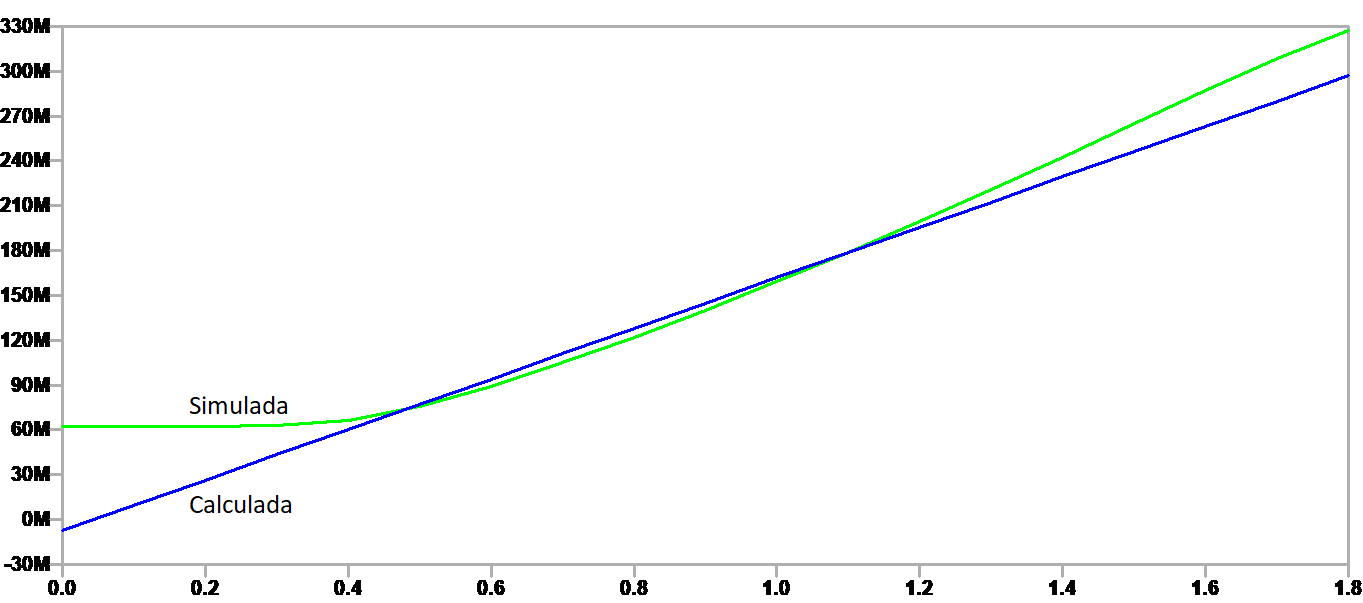
\includegraphics[scale=0.4]{./img/vco7_sim}
\caption{Simulación de Frecuencia medida y estimada contra $V_{IN}$.}
\label{fig:vco7_sim}
\end{figure}

\section{Divisor de Frecuencias}

\section{PFD}

\section{PFD PLLD}




TODO higher gain VCO, add pre scalar and post scalar. Simulations of

100 MHz input clock div 4, mul 6, div 2 to get 75 MHz


\begin{thebibliography}{9}

\bibitem{RBaker}
R. Jacob Baker (2010) \emph{CMOS: Circuit design, layout and simulation}, Wiley-IEEE Press, 3rd edition.

\bibitem{vco}
Suman, Shruti \& G Sharma, K \& Ghosh, Pradip. (2016). \emph{Analysis and Design of Current Starved Ring VCO}. 10.1109/ICEEOT.2016.7755299.

\end{thebibliography}

\end{document}